% !TeX root = ../msc-thesis.tex
\documentclass[../msc-thesis.tex]{subfiles}

\begin{document}

\chapter{\mtc practice and recommendations}
\label{section:discussion}

In this chapter will be done a thorough discussion of usage aspects of \mtc, 
recommendations and good-practices when using the proposed software. 
The main idea is to pass to the reader a concise set of recommendations and 
the justification for these. The covered aspects will be mainly:

\begin{enumerate}
    \item The process simulator sampling general good practice: Towards 
    maximizing cases convergence while keeping precision;

    \item The initial sample: Dimensionality and the choice of the degrees of 
    freedom towards the optimization feasible region;

    \item The adaptive sampling optimization algorithm parameters;

    \item The reduced-space problem sample: Dimensionality and the effect of 
    the \textcite{Lophaven2002} hyperparameters objective function in 
    gradient/hessian evaluation.
\end{enumerate}

\section{The process simulator sampling general good practice:  Towards 
maximizing cases’ convergence while keeping precision}

When one is using a modular flowsheet process simulator, such as Aspen Plus, 
problems will eventually arise based on model complexity and the necessity
of realistically representing a process becomes of utmost importance. Unit 
operations such as distillation and chemical reactors are sources of numerical 
noise, result of termination criteria in the algorithms that solve these unit 
operations blocks, or even rounding numbers, as discussed by 
\textcite{Caballero2008}. With this problem, some workarounds are suggested 
in order to try to reduce the number of unconverged cases and to enhance 
precision. The problem gets even more complicated when recycle streams are 
present in the process, acting as noise-amplifiers \cite{Quirante2016}. 
With the aforementioned problems being stated, some recommendations that 
worked well based on the study of previous publications are:

\begin{enumerate}
    \item Tighten as much as possible the following convergences' tolerances: 
    tear stream-related, Inside/Out algorithm for distillation blocks-related, 
    and chemical reactors' convergence related. Mixers, pumps and heat-exchangers 
    were previously shown to not introduce - or introduce irrelevant - noise 
    \cite{Quirante2016}.

    \item \textcite{Aspentech2017} recommends that when a tear streams/recycle 
    streams are present in the flowsheet interacting with distillation column 
    blocks, the convergence tolerance of the former should be at least a 
    order of magnitude lower (tighter) than the latter. This will avoid the 
    numerical noise from the distillation block to impede convergence.

    \item Reconcile the tear streams. When these streams are reconciled, 
    there are input specifications inside those that will aid the convergence. 
    In fact, the number of cases converged increased when the authors of this 
    work reconciled the flowsheet with a feasible operating point. The 
    procedure to reconcile the tear streams can be found in 
    \textcite{Aspentech2017}.

\end{enumerate}

\section{The initial sample: Dimensionality and the choice of the degrees of 
freedom towards the optimization feasible region} \label{subsection:point2}

In order to successfully obtain a nominally optimal operating point, one must 
ensure that the initial sample provided to the algorithm proposed by 
\textcite{Caballero2008} it is capable of representing the basic trends of the 
objective function and the nonlinear constraints created by the user. However, 
the so called ``curse of Dimensionality'' \textcite{Forrester2008} still looms 
over big-data and machine-learning fields of study. The dimensionality can 
be reduced using engineering common sense, as different authors did in the 
past for instance \cite{Araujo2007,Araujo2008,Gera2013}. 

The idea is to keep constant the degrees of freedom that have little or no 
effect on the objective function, and, instead, use only the degrees of 
freedom that are ``dominant'' in the process. Another way of reducing the 
number of degrees of freedom is to anticipate results that are expected to 
be active constraints, specially when one is dealing with economic \soc. 
Strictly speaking: one can expect active constraints in liquid-phase reactor's 
maximum holdups and temperatures, when the kinetics are simple; maximum 
operating pressure for gas-phase reactors, minimum acceptable purity for 
valuable products (avoiding product ``giveaway'' \cite{Jacobsen2011}) and 
maximum impurity levels in contaminants restrictions all expected to occur, 
for instance. These results were repeatedly found over several years of \soc 
studies, and were synthesized in the work of \textcite{Minasidis2015}.

Regarding the number of points in the initial sample, this problem it is a 
heuristic one. If the number of points is too low, the prediction capability of 
the metamodel decreases, and the optimal solution found before the contraction 
steps could be far from the actual solution, and several movement steps would 
be necessary, consuming time \cite{Caballero2008}. In addition, the number of 
points as discussed by \textcite{Caballero2008} is case-dependent: For instance, 
given a function with a sharp peak, it will require a large number of points 
around it. However, using an excessively amount of points can be time consuming 
(if each model evaluation takes considerable time and due to matrix inversion 
operations performed by the \textit{pydace} toolbox) or even worse, starting 
ill-conditioning the correlation matrix $R$, if the large amount of points are 
not separated enough (new points introduced can be clustered and making $R$ 
ill-conditioned). This can also jeopardize the \kriging metamodel construction 
and consequently, its prediction capability.

In order to balance accuracy and number of points, the authors of this work use 
as a starting point the heuristic proposed by \cite{Caballero2008}: around 
30-50 points for two or three variables, around 70-80 for four/five variables, 
and increasing by 10 points for each additional independent variable. The work 
of \textcite{Caballero2008} uses the maximum practical limit of 100 points. 
However, some cases might need more points than this limit, and the reader 
should not feel inhibited of trespassing this limit. Nevertheless, he must be 
careful with the excess of points, due to the reasons aforementioned.

Lastly, regarding the degrees of freedom chosen to perform the design of 
experiments, it has been shown by previous authors \textcite{Hori2005,
Kariwala2008} that any variable can be chosen as a degree of freedom, since 
the problem is evaluated in steady-state, there is no loss of generality.
Therefore, one can try to convert the nonlinear constraints, for instance, 
to decision variables (box constraints). This will enforce that all the sampled 
(and converged) cases, to be inside the feasible region of the optimization 
problem. To use design specifications/constraints as decision variables is 
not a new approach and it has been done in the past \textcite{Gera2013,
Jagtap2013} when the cited authors were using a NLP solver coupled with the 
process simulator, trying to ensure robust convergence of the optimization 
problem. As an example, if one chooses to sample the purity of a valuable 
product from a distillation column instead of a reflux rate, he not only 
knows automatically the bounds of that variable $x_{min} \leq x \leq 1$, but 
all of the sampled cases would be within the optimization problem feasible 
region.

\section{The adaptive sampling optimization algorithm parameters}

The contraction factors (namely \textit{first} and \textit{second}), 
refinement, termination and \textit{maximum contraction} tolerances can be 
tuned in order to achieve a quicker optimization convergence. As discussed by 
\textcite{Caballero2008}, using a large value for the \textit{first} 
contraction factor might result in a increased amount of hypercube movements, 
even though the final result will be the same. As a general setup, the 
parameters values are 0.6 and 0.4 for \textit{first} and \textit{second} 
factors, respectively.

The termination parameter value, as a rule of thumb, is set to be at least a 
order of magnitude higher than the tightest convergence parameter set in the 
process simulator, so that the optimization procedure does not adjust the 
numerical noise introduced by the simulation software. Then the refinement 
parameter is set to be at least one order of magnitude higher than the 
termination value.

However, care must be taken when specifying the \textit{maximum contraction} 
factor, since this parameter tells the algorithm the minimum hypercube size to 
contract. This a safeguard parameter to prevent the introduction of 
ill-conditioning in the \kriging input matrix. Consequently, this parameter 
cannot be higher than the refinement value.

\section{The reduced-space problem sample: Dimensionality and the effect of 
the \kriging hyperparameters objective function in gradient/hessian 
evaluation.}

When one is obtaining high-order data using kriging metamodels, he must be aware 
of the value of the $\psi$ objective function that is minimized using the 
hyperparameters as degrees of freedom (\Cref{eq:kr6}). It has been found that 
convergence values that are acceptable for general prediction purposes 
(i.e.: $10^{-3}$ to $10^{-4}$) are not suitable to predict the gradients and 
hessians necessary to the SOC study. Regarding the hessians 
$(\left(\frac{\partial^{2} J}{\partial u \partial d}\right)$, 
$\left(\frac{\partial^{2} J}{\partial u \partial u}\right))$, they are even more 
sensitive to the hyperparameters estimation (an expected result, due to the fact 
that they are second derivatives). It was found that a good value for 
the $\psi$ function that was capable of generating metamodels that are capable 
of predicting the gradients and hessians with precision, would be around 
$10^{-5}$ (at least). This variable can be inspected within \mtc, 
under the panel ``Validation metrics'', for the reduced-space metamodel, as can 
be seen in \Cref{fig:perf}. Its value can be used as a metric of how 
precise the gradient and hessian evaluation will be. As showed in the previous 
examples when for illustration purposes the original gradient was evaluated, 
the agreement between the metamodel-based gradient and the original one is 
excellent.

\begin{figure}[htb]
    \centering
    \caption{$\psi$ function value - named ``perf'' within \mtc.}
    \label{fig:perf}
    \makebox[1.0\textwidth]{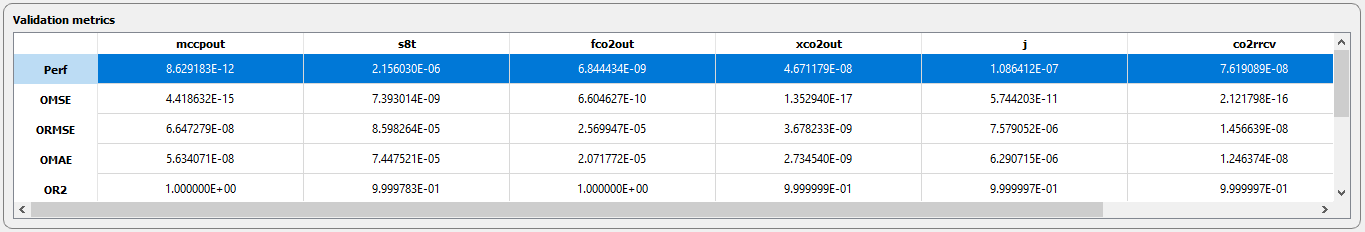
\includegraphics[width=1.0\textwidth]
    {perf_good.PNG}}
\end{figure}

\FloatBarrier
\end{document}